\documentclass[Journal,letterpaper, SingleSpace]{ascelike-new}
%\usepackage{etex}
%\newcommand{\num}{6{} }

%\raggedbottom

%geometry (sets margin) and other useful packages
% \usepackage{geometry}
% \geometry{top=1.2in, left=1in,right=1in,bottom=1in,headsep=6pt}
\usepackage{graphicx,booktabs, calc}

%=== GRAPHICS PATH ===========
\graphicspath{{./figures/}}
% Marginpar width
%Marginpar width
% \newcommand{\pts}[1]{\marginpar{ \small\hspace{0pt} \textit{[#1]} } }
% \setlength{\marginparwidth}{.5in}
%\reversemarginpar
%\setlength{\marginparsep}{.02in}

%% Fonts
% \usepackage{fourier}
% \usepackage[T1]{pbsi}
%\usepackage[utf8]{inputenc}
\usepackage[T1]{fontenc}
\usepackage{lmodern}
%\usepackage{minted}
\usepackage[figurename=Fig.,labelfont=bf,labelsep=period]{caption}
\usepackage{subcaption}
\usepackage{amsmath}
%\usepackage{rotating}
\usepackage{newtxtext,newtxmath}
\usepackage[colorlinks=true,citecolor=red,linkcolor=black]{hyperref}


%% Cite Title
%\usepackage[style=numeric,backend=biber,natbib,sorting=none,maxcitenames=2,maxbibnames=99,doi=false,isbn=false,url=false,eprint=false]{biblatex}
%\addbibresource{../ai-trees-references.bib}

%%% Counters
% \usepackage{chngcntr,mathtools}
% \counterwithout{figure}{section}
% \counterwithout{table}{section}

% \numberwithin{equation}{section}

% %% Captions
% \usepackage{caption}
% \captionsetup{
%   labelsep=quad,
%   justification=raggedright,
%   labelfont=sc
% }

%AMS-TeX packages
%\usepackage{amssymb,amsmath,amsthm}
%\usepackage{bm}
%\usepackage[mathscr]{eucal}
%\usepackage{colortbl}
%\usepackage{color}

%\DeclareRobustCommand{\hlcyan}[1]{{\sethlcolor{cyan}\hl{#1}}}

\usepackage{enumerate}


\usepackage{multirow,array,multicol}

%
%\definecolor{slblue}{rgb}{0,.3,.62}
% \hypersetup{
%     colorlinks,%
%     citecolor=blue,%
%     filecolor=blue,%
%     linkcolor=blue,
%     urlcolor=slblue
% }

%%%TIKZ
% \usepackage{tikz}
% \usepackage{pgfplots}
% \usepackage{pgfplotstable}
% \usepackage{pgfgantt}
% \pgfplotsset{compat=newest}

% \usetikzlibrary{arrows,shapes,positioning}
% \usetikzlibrary{decorations.markings}
% \usetikzlibrary{shadows,automata}
% \usetikzlibrary{patterns,fit}
% %\usetikzlibrary{circuits.ee.IEC}
% \usetikzlibrary{decorations.text}
% % For Sagnac Picture
% \usetikzlibrary{%
%     decorations.pathreplacing,%
%     decorations.pathmorphing%
% }


% \newcommand{\osn}{\oldstylenums}
% \newcommand{\dg}{^{\circ}}
% \newcommand{\lt}{\left}
% \newcommand{\rt}{\right}
% \newcommand{\pt}{\phantom}
% \newcommand{\tf}{\therefore}
% \newcommand{\?}{\stackrel{?}{=}}
% \newcommand{\fr}{\frac}
% \newcommand{\dfr}{\dfrac}
% %\newcommand{\ul}{\underline}
% \newcommand{\tn}{\tabularnewline}
% \newcommand{\nl}{\newline}
% \newcommand\relph[1]{\mathrel{\phantom{#1}}}
% \newcommand{\cm}{\checkmark}
% \newcommand{\ol}{\overline}
% \newcommand{\rd}{\color{red}}
% \newcommand{\bl}{\color{blue}}
% \newcommand{\pl}{\color{purple}}
% \newcommand{\og}{\color{orange!90!black}}
% \newcommand{\gr}{\color{green!40!black}}
% \newcommand{\nin}{\noindent}
% \newcommand{\la}{\lambda}
% \renewcommand{\th}{\theta}
% \newcommand{\al}{\alpha}
% \newcommand{\G}{\Gamma}
% \newcommand*\circled[1]{\tikz[baseline=(char.base)]{
%             \node[shape=circle,draw,thick,inner sep=1pt] (char) {\small #1};}}


% \newcommand{\p}{\partial}
% \newcommand{\pd}[2]{\frac{\partial{#1}}{\partial{#2}}}
% \newcommand{\dpd}[2]{\dfrac{\partial{#1}}{\partial{#2}}}
% \newcommand{\pdd}[2]{\frac{\partial^2{#1}}{\partial{#2}^2}}


%%%%%%%%%%%%%%%%%%%%%%%%%%%%%%%%%%%%%%%%%%%%%%%%%%%
%%%%%%%%%%%%%%%%%%%%%%%%%%%%%%%%%%%%%%%%%%%%%%%%%%%
\NameTag{Author1LastName, \today}

\begin{document}
% ALL CAPS TITLE REQUIRED
\title{Predicting tree failure likelihood for utility risk mitigation via a novel convolutional neural network}
\author[1]{Author 1}
\author[2]{Author 2}
\author[2]{Author 3}
\author[2]{Author 4}
\author[2]{Author 5}

\affil[1]{First affiliation address, with corresponding author email. Email: author.one@umass.edu}
\affil[2]{Second affiliation address}

\maketitle

\begin{abstract}
    Abstract here.
\end{abstract}

\section{Introduction}
Power outages due to contact between tree parts and power lines annually cause tens of billions of dollars in economic and other disruptions throughout the United States, despite extensive efforts by utilities to mitigate and prevent those contacts.  Presently, the identification of potential contact between trees and power lines is labor intensive and time-consuming.  This paper describes an artificial intelligence and machine learning approach that automatically classifies trees, using only a single photograph and with a high degree of accuracy, into categories corresponding to probable failure, possible failure and improbable failure-categories corresponding to those used by utility arborists to assess risk of contact between trees and power lines.  This preliminary study demonstrates the possible efficacy of AI approaches to tree risk assessment and, following further development of the approach has the potential to reduce power outages and utility costs by allowing utilities to more effectively target their pruning and mitigation efforts.  

Contact between tree parts and power lines can take several forms: tree branches can grow into lines; branches can fail and fall onto lines; whole-tree failure can occur due to uprooting or trunk failure.  A study in the state of Connecticut, USA provides some context for the amount of economic disruption, documenting annual disruptions of \$8.3 billion between 2005 and 2015 \cite{graziano2020wider}.  That extremely high cost occurred despite extensive efforts on the part of utilities to mitigate conflicts between trees and power lines through active and aggressive pruning programs that, on their own cost billions of dollars annually \cite{guggenmoos2003effects}.  

Pruning, despite its high cost, has been found to be effective in reducing disruptions due to so-called ``preventable'' contact incidents between trees and power lines.  For example, in Massachusetts, USA, where tree failure was responsible for 40\% of preventable tree-caused outages, pruning was able to improve reliability by 20\% to 30\% \cite{simpson1996treecaused}, and those results were replicated in a study in Connecticut \cite{parent2019analysis}. The efficacy of pruning has also been shown in a study of two states in the Gulf Coast region of the USA that showed wind-induced power outage prediction models becoming less uncertain when pruning was included in the model \cite{nateghi2014power}.

Even effective pruning cannot, however, completely eliminate tree-caused outages. Failure of trees away from the right-of-way can still impact the lines and cause outages \cite{guggenmoos2003effects}. The proportion of tree failures away from the wires that causes outages varies and has not been rigorously quantified. \citeN{guggenmoos2011treerelated} estimated that 95\% of tree-caused outages in the Pacific Northwest region of the USA, were due to tree failure, and \citeN{wismer2018targeted} reported approximately 25\% of interruptions in Illinois, USA, were caused by trees that uprooted or broke in the stem. 


Predicting the likelihood of failure is an inexact science, but tree risk assessment best management practices have been developed \cite{smiley2017best,goodfellow2020best}. Risk includes assessing the likelihood of failure, the likelihood of impact, and the severity of consequences. The likelihood of failure depends on the anticipated loads on the tree and its load-bearing capacity. The likelihood of impact depends on proximity to the target (the lines, poles, and other hardware---``infrastructure''---in the case of utility tree risk assessment), the target’s occupancy rate (which is constant for utility lines) and whether the target is sheltered, for example by neighboring trees. Severity of consequences depends on the damage done to the infrastructure---which, in turn, is partially related to the size of the tree or tree part that fails, and how much momentum it has when it impacts the infrastructure---and, more importantly in some cases, the economic costs and disruption associated with outages.

Individual tree risk assessment can be costly because of the time it requires. In some situations, a less time-consuming assessment may be justified to reduce costs, i.e.\ a ``Level 1'' assessment  \cite{smiley2017best}. Studies have shown that trees with greater risk ratings were more likely to be detected from Level 1 risk assessments conducted in a moving vehicle in Rhode Island, USA \cite{rooney2005reliability} and Florida, USA \cite{koeser2016frequency}. The utility of Level 1 assessments in these states suggests that artificial intelligence (AI) tools may be an effective way to reduce the cost of tree risk assessment.

The method described in the paper uses convolutional neural networks (CNN) to classify images of trees among three categories of failure likelihood: probable, possible, and improbable.  The data used for training, testing and illustration of the method consists of 505 tree images that have been classified by the authors according to prevailing standards employed by professional utility arborists. 

The remainder of the paper provides a brief history and background of AI and its use in earthquake risk assessment and tree identification (section 2); describes the methods used to train and validate a novel CNN to categorize likelihood of tree failure (section 3); and presents and discusses the output of the novel CNN (sections 4 and 5). The goal is to further demonstrate an innovative automated approach to tree risk assessment using an AI tool that can be readily deployed for use in various locations and also continually improved through subsequent training on new datasets.



\section{Background}

%\subsection{AI and risk assessment}
AI-based image analysis is relatively widely used, even in engineering applications, such as earthquake risk assessment \cite{jiao2020artificial,salehi2018emerging} and structural health monitoring \cite{spencer2019advances}. Neural networks have been widely applied in the field of earthquake risk assessment (an excellent review is provided by \citeN{xie2020promise}), but the authors are not aware of attempts to operate directly on, for example, building images in the absence of technical structural data to predict seismic risk.  Neural networks have also been used to interrogate remote sensing data of the landscape to assess landslide risk \cite{su2020deep}.


A relevant application for tree species identification using a convolutional neural network (CNN) was recently demonstrated \cite{fricker2019convolutional}. Yet, AI has not been applied to the problem of tree-utility line risk assessment---one that is complicated by the very large number of tree species to be considered, seasonal variation in tree appearance and associated risk and local meteorological conditions. 


%Neural networks developed over the past several decades from the introduction of the single-layer perceptron.
The groundbreaking study of \citeN{hubel1959receptive} showed that visual perception in cats was a result of the
activation or inhibition of groups of cells in the visual cortex known as ``receptive fields.''  Further, they attempted
to map the cortical architecture in cats and monkeys \cite{hubel1962receptive,hubel1965receptive,hubel1968receptive}.
Subsequent attempts were then made to model neural networks that could be trained to automatically recognize visual patterns with modest performance \cite{rosenblatt1962principles,kabrisky1966proposed,giebel1971feature,fukushima1975cognitron}. However, the breakthrough came with the ``neocognitron'' \cite{fukushima1980neocognitron}, which
was a self-learning neural network for pattern recognition that was robust to changes in position and shape distortion, a problem that plagued earlier efforts, including ``cognitron'' \cite{fukushima1975cognitron} proposed a few years earlier.

A few notable efforts demonstrated the neural networks for handwritten digit recognition
\cite{fukushima1988neocognitron,denker1988neural}, but these required significant preprocessing and feature
extraction. \cite{lecun1989handwritten} soon afterward introduced a multilayer neural network that mapped a feature in each neuron (representing a ``local receptive field'') via convolution. This network could also be trained by backpropagation like other existing neural networks and featured pooling operations for better distortion and
translation invariance. Further developments from this milestone yielded the LeNet-5 convolutional neural network which attained accuracy levels that rendered it commercially viable.

The big data revolution coupled with technological advancements that have made it possible to capture and store high resolution images have raised challenges that continue to be surmounted with successively high-performing
architectures. Over the past decade, some of these efforts resulted in significant breakthroughs in performance. AlexNet \cite{krizhevsky2012imageneta}, with 5 convolutional layers and 3 dense layers---one of the largest CNNs of its time, won the ILSVRC-2012\footnote{ImageNet Large Scale Visual Recognition Challenge; held annually from 2010 through 2017.} competition with a top-5 error rate of 15.3\% and served as a landmark in the Deep Learning subdomain. \citeN{zeiler2014visualizing} then introduced ZFNet, besting the performance of AlexNet, and pioneered visualization techniques that were foundational for model inference and interpretability.  In the same year, GoogLeNet, a 22-layer network, was proposed \cite{szegedy2014going}, featuring the novel ``Inception module,'' which allowed for efficiency and accuracy in a very deep network. Subsequent improvements have been proposed to the original inception framework \cite{szegedy2015rethinking,szegedy2016inceptionv4}.  VGGNet \cite{simonyan2015very} also pushed the boundaries of depth with up 19 layers, achieving state-of-the-art performance at ILSVRC-2014. Finally, ResNet \cite{he2015deep} addressed the accuracy degradation problem that arises with increasing depth in a network by successively fitting smaller sets of layers to the residual and employing skip connections. With these innovations, an unprecedented level of depth was achieved. Implementations with with 34, 50, 101 and 152 layers were demonstrated. ResNet-152 won first place in ILSVRC-2015.

Along with these developments in their architectures, CNNs have demonstrated viability for applications to image
classification, object and text detection, object and document tracking, labeling, speech, among several other related
fields \cite{gu2018recent}. %\hl{Paragraph on applications to be completed---with particular attention paid to tree-related efforts.}


\section{Data and Methods}
\subsection{Image data description}
The training dataset consisted of 505 images, each having an original size of $4032\times3024$ pixels.   Images were captured over a single field season in Massachusetts, USA, between May and September 2020 to limit any potential influence of changes in tree appearance due to seasonal leaf senescence on image processing.  ESRI ArcMaps was used to randomly distribute sampling sites across the state.  Likelihood of failure assessments followed the “Level 1” methods outlined in the second edition of the International Society of Arboriculture’s (ISA) Tree Risk Assessment Best Management Practices \cite{smiley2017best} and ISA’s Utility Tree Risk Assessment Best Management Practices \cite{goodfellow2020best}.  This method is commonly used to assess trees in the United States.  A level 1 assessment was selected for this study because: (1) individual risk assessments may be prohibitively expensive at higher orders, i.e. Level 2 or Level 3 \cite{smiley2017best}, given the hundreds of thousands of trees utilities must manage across territory areas;  (2) utility rights-of-way (ROW) easements may not allow utility inspectors full access to trees in practical application of higher order risk assessment procedure if the trees are beyond the edge of the ROW \cite{goodfellow2020best}; (3) studies have shown reasonable efficacy of limited basic visual assessment techniques in identifying more severe tree defects \cite{rooney2005reliability,koeser2016frequency} leading to greater likelihood of failure ratings.  The four categories of likelihood of tree failure, which are always considered in a stated time frame, are defined as follows \cite{smiley2017best}:
\begin{itemize}
\item \textbf{Improbable}: failure unlikely either during normal or extreme weather conditions 
\item \textbf{Possible}: failure expected under extreme weather conditions; but unlikely during normal weather conditions
\item \textbf{Probable}: failure expected under normal weather conditions within a given time frame
\item \textbf{Imminent}: failure has started or is most likely to occur in the near future, even if there is no significant wind or increased load. This is a rare occurrence for a risk assessor to encounter, and may require immediate action to protect people from harm
\end{itemize}
In this study, only images of trees assigned to the lowest 3 likelihood of failure categories of \textit{improbable, possible, \textit{and} probable} were used due to the rarity of trees in the \textit{imminent} category. Two randomly chosen examples are shown for each category in \autoref{fig:raw_images}.   

\begin{figure}[h!]
  \centering
  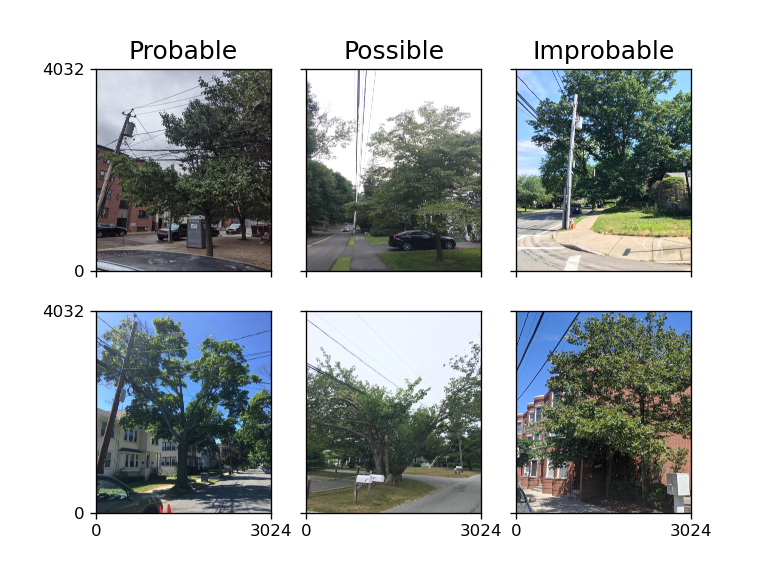
\includegraphics[width=.7\textwidth]{raw_input_images_2}
  \caption{Random examples of the raw training images (2 are shown per class). Images are antialiased in this figure for greater clarity.}
  \label{fig:raw_images}
\end{figure}

\subsection{Pre-processing and data augmentation}
In the original set of training images, the class distribution is given in \ref{tab:classdist}.

\begin{table}[h!]\small
    \centering
    \begin{tabular}{l l}\toprule
    \bf Class Label     & \bf Number of images  \\ \midrule
    Improbable & 322\\
    Possible & 80 \\
    Probable & 56 \\\midrule
    Total & 505 \\\bottomrule
    \end{tabular}
    \caption{Class distribution of images in training set}
    \label{tab:classdist}
\end{table}

To achieve robustness in training, and given the relatively small number of training images, we randomly cropped each image on either axis to 3024 $\times$ 3024 pixels, generating five instances for each one. Thus, we increased the size of our training set from 505 to 2525 images. Further, we performed horizontal flipping with a 50\% probability on each of the generated images. For efficiency, we converted the images to grayscale and scaled the pixel values from 0 to 1. Finally, we downsampled the images to the following resolutions: $64 \times 64$, $128 \times 128$, $224 \times 224$ and $384\times 384$, creating a training set for each case. 

\begin{figure}[h!]
  \centering
  \begin{subfigure}[t]{.5\linewidth}
    \centering
    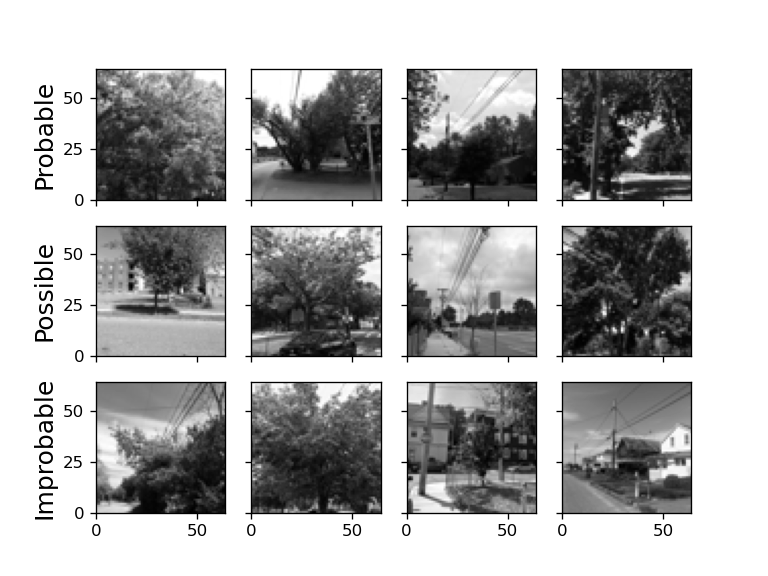
\includegraphics[width=\linewidth]{processed_input_images_Pr_Po_Im_64_px}
    \caption{Scenario \texttt{Pr\_Po\_Im}}
    \label{pr_po_im_64}
  \end{subfigure}%
  \begin{subfigure}[t]{.5\linewidth}
    \centering
    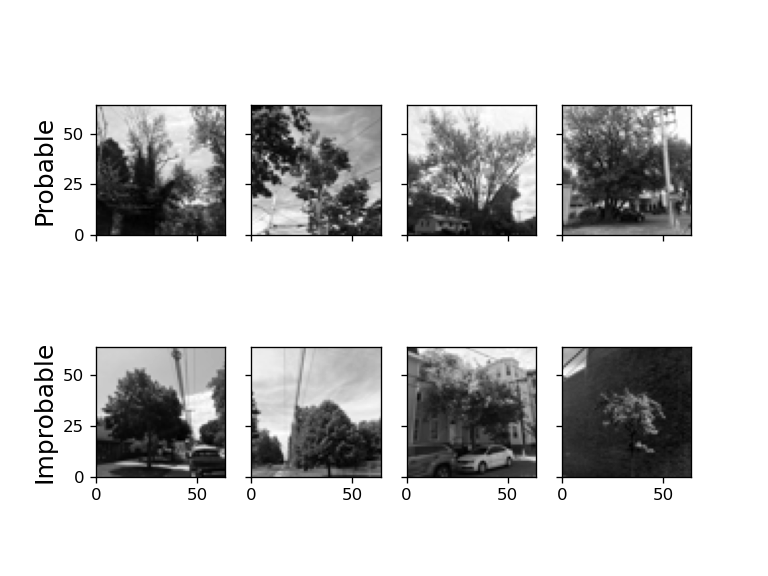
\includegraphics[width=\linewidth]{processed_input_images_Pr_Im_64_px}
    \caption{Scenario \texttt{Pr\_Po\_Im}}
    \label{pr_im_64}
  \end{subfigure}%
  
  \begin{subfigure}[t]{.5\linewidth}
    \centering
    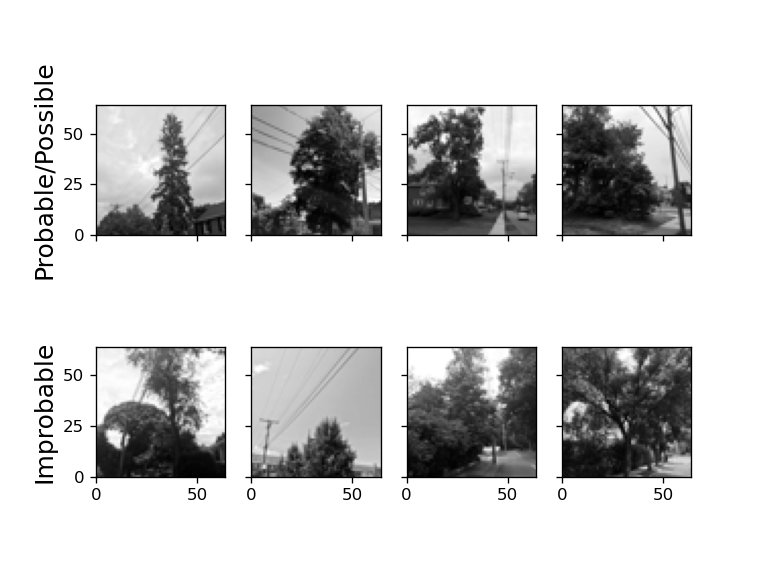
\includegraphics[width=\linewidth]{processed_input_images_PrPo_Im_64_px}
    \caption{Scenario \texttt{Pr\_Po\_Im}}
    \label{prpo_im_64}
  \end{subfigure}%
  \begin{subfigure}[t]{.5\linewidth}
    \centering
    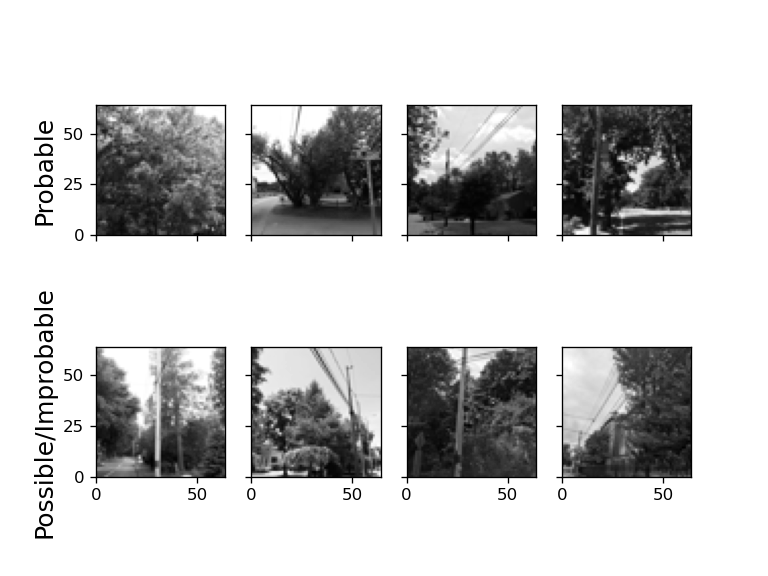
\includegraphics[width=\linewidth]{processed_input_images_Pr_PoIm_64_px}
    \caption{Scenario \texttt{Pr\_Po\_Im}}
    \label{pr_poim_64}
  \end{subfigure}%

  \caption{Random examples of the processed training images under each classification scenario; 64 pixels.}
  \label{fig:processed_images}
\end{figure}

\subsection{Convolutional neural network}

We can apply cut-out (occluding portions of the image) for improved performance \cite{devries2017improved}. Also, it has been shown that training with lower resolution improves performance on higher resolution test images \cite{touvron2019fixing}.


\subsection{Hyperparameter optimization}
We used the Hyperband approach \cite{li2018hyperband} to perform a grid search to find the optimal values of the following hyperparameters:
\begin{itemize}
    \item kernel size in first convolutional layer
    \item number of units in first densely connected layer
    \item dropout rate applied to outputs of first dense layer
    \item activation function for first dense layer
    \item number of units in second densely connected layer
    \item dropout rate applied to outputs of second dense layer
    \item activation function for second dense layer    
    \item learning rate (of Adam optimizer)
\end{itemize}

\section{Results}

\subsection{Classification experiments}

We define four classification scenarios in \ref{tab:scenarios}. 

\begin{table}[h!]
    \centering
    \begin{tabular}{l l l}\toprule
    \bf Scenario            & \bf Description  & \bf No.\ classes\\\midrule
    \texttt{Pr\_Po\_Im}     &  \{Probable, Possible, Improbable\} & 3 \\
    \texttt{Pr\_Im}          & \{Probable, Improbable\}           & 2 \\
    \texttt{PrPo\_Im}        & \{Probable|Possible, Improbable\}  & 2 \\
    \texttt{Pr\_PoIm}        & \{Probable, Possible|Impossible\}  & 2 \\\bottomrule
    \end{tabular}
    \caption{Classification scenarios}
    \label{tab:scenarios}
\end{table}

\subsection{Sensitivity to training resolution}

\subsection{Model visualization and inference}

\subsection{Comparison with state-of-the-art architectures}
We compare the performance of our selected model with existing high-performance architectures. The results are summarized in \ref{tab:comp}.

\begin{table}[h!]\small
  \centering
  \begin{tabular}{l l l l l l l }\toprule
    \bf Model & \multicolumn{3}{c}{\bf Training metrics} &\multicolumn{3}{c}{\bf Validation metrics}  \\\midrule
    & Error & Precision & Recall     & Error & Precision & Recall \\
    SafeTree & & & & & & \\
    GoogleNet (InceptionV3) & & & & & & \\
    ResNet50 & & & & & & \\
        VGGNet & & & & & & \\
    AlexNet & & & & & & \\\bottomrule
  \end{tabular}
  \caption{Comparing our model SafeTree with state-of-the-art CNN architectures trained on our data}
  \label{tab:comp}
\end{table}
\section{Conclusion}

\section{Data Availability Statement}
All data, models, or code generated or used during the study are available in a repository online in accordance with funder data retention policies (provide full citations that include URLS or DOIs)

Please also see the guidelines at: \url{https://ascelibrary.org/page/dataavailability}.

\section{Acknowledgments}

\appendix

\bibliography{ai-trees-references}   



\end{document}

 
%%% Local Variables:
%%% mode: latex
%%% TeX-master: t
%%% End:
